\section{Estereótipo OpenAccess}

Ao criar aplicações utilizando o MDArte, é oferecido ao usuário a opção de
utilizar a camada de segurança já implementada no MDArte. Ao escolher essa
opção, a aplicação MDArte só poderá ser acessada por usuários cadastrados.
Contudo, exitem aplicações em que o acesso público a algumas páginas da é
um requisito.

Para tornar a página pública você deve atribuir o estereótipo
\texttt{OpenAccess} ao caso de uso referente a página ou ao pacote que contém o caso de uso. Atribuir o
estereótipo a pacotes acima dos que tem os estereótipos \texttt{ModuloWeb} ou
\texttt{ModuloWebPai} não tornará a página pública pois o sistema finaliza a
checagem até pacotes com estes estereótipos.

O esetereótipo \texttt{OpenAccess} também é aplicado em pacotes da camada de
serviço. Isso é devido a casos de páginas públicas precisarem utilizar serviços
de acesso a banco de dados sem precisarem se logar. O estereótipo
\texttt{OpenAccess} deve ser aplicado em pacotes com estereótipo
\texttt{ModuloServico}

\begin{figure}[H]
	\centering
	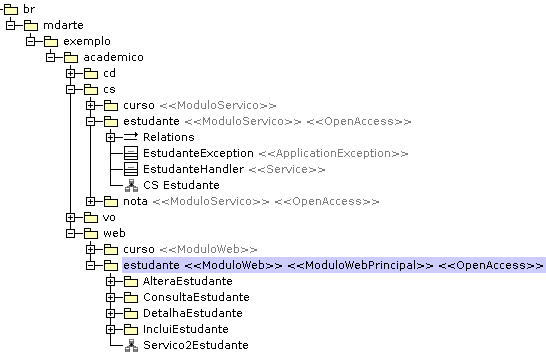
\includegraphics[width=350pt,height=300pt]{files/imgs/openaccess-00.png}
	\caption{Exemplo de uso do estereótipo OpenAccess.}
	\label{open_access}
\end{figure}

No exemplo acima, todos os casos de uso do pacote \texttt{estudante} são
públicos. Se aplicasse o estereótipo no pacote \texttt{web} nada aconteceria. Se fosse apenas no pacote
\texttt{consultaPais}, apenas esse caso de uso seria público. Além disso, os
serviços dos pacotes \texttt{estudante} e \texttt{nota} são públicos.
